\documentclass[12pt]{article}

\usepackage{fullpage}
\usepackage[spanish]{babel}
\usepackage{amsfonts} %for double trace letters
\usepackage{amssymb}
\usepackage{amsmath} %for special/unusual mathematical characters
\usepackage{eufrak} %for gothic letters
\usepackage{graphicx} %Image includer package
\graphicspath{{Images/}} %Image directory
\usepackage{xcolor}

\usepackage{multicol} %For writing text in columns
\setlength{\columnsep}{1cm} %Defines separation of columns

\usepackage{tcolorbox} %for boxes that enclose text
\usepackage{color}
\definecolor{myblue}{rgb}{.8, .8, 1}

\usepackage{empheq}

\newlength\mytemplen
\newsavebox\mytempbox

\makeatletter
\newcommand\mybluebox{%
    \@ifnextchar[%]
       {\@mybluebox}%
       {\@mybluebox[0pt]}}

\def\@mybluebox[#1]{%
    \@ifnextchar[%]
       {\@@mybluebox[#1]}%
       {\@@mybluebox[#1][0pt]}}

\def\@@mybluebox[#1][#2]#3{
    \sbox\mytempbox{#3}%
    \mytemplen\ht\mytempbox
    \advance\mytemplen #1\relax
    \ht\mytempbox\mytemplen
    \mytemplen\dp\mytempbox
    \advance\mytemplen #2\relax
    \dp\mytempbox\mytemplen
    \colorbox{myblue}{\hspace{1em}\usebox{\mytempbox}\hspace{1em}}}

% for theorems
\usepackage{amsthm}
 
\theoremstyle{definition}
\newtheorem{definition}{Definici\'on}[section]

\theoremstyle{theorem}
\newtheorem{theorem}{Teorema}[section]

\theoremstyle{corolary}
\newtheorem{corolary}{Corolario}[section]

\DeclareMathOperator{\Arg}{Arg}
\DeclareMathOperator{\Log}{Log}
\DeclareMathOperator{\sen}{sen}
\DeclareMathOperator{\senh}{senh}
\DeclareMathOperator{\tg}{tg}
\DeclareMathOperator{\ctg}{ctg}
\DeclareMathOperator{\tgh}{tgh}
\DeclareMathOperator{\ctgh}{ctgh}
\DeclareMathOperator{\sech}{sech}
\DeclareMathOperator{\csch}{csch}



\begin{document}
	\title{Derivaci\'on Compleja}
	\author{Breggia, Bruno M.}
	\date{}
	\maketitle

Se conocen ya algunas funciones de variable compleja, o varias, mejor dicho. ?`C\'omo convertir esto en la mejor arma matem\'atica para modelar al Universo? Pues, si somos capaces de calcular tasas de cambio con ellas, tenemos al Universo en nuestras manos. Pues en \'el, la \'unica constante es el cambio (dice un proverbio chino). Es por ello que en esta lecci\'on nos introduciremos a la \textbf{diferenciaci\'on} de funciones de variable compleja. ?`Qu\'e tan distinto puede ser...?\\ \\

\begin{center}
	
\includegraphics[scale=1.4]{glass2.jpg}
\end{center}

\pagebreak
\tableofcontents
\pagebreak

\section{Definimos la derivada compleja}
Ya sabemos lo que es la derivada, representa la tasa de cambio de una magnitud respecto a alguna variable de la que depende. Pero cuando hablamos de funciones de variable compleja, la intuici\'on geom\'etrica de que la derivada representa la pendiente de la curva ya no se da tan as\'i... pues las funciones complejas no pueden representarse en un mismo plano con su conjunto dominio. Y ojo, que adem\'as cualquier noci\'on de pendiente y velocidad que le podr\'iamos asociar se distorsiona con asignarles como valor alguna cantidad compleja...

Sin perdernos entonces en una interpretaci\'on geom\'etrica de la misma, le daremos a la derivada de funciones complejas una nueva definici\'on, que ser\'a an\'aloga a la que conoc\'iamos para funciones de una varible real (e inclusive similar a la de funciones vectoriales $\mathbb{R}^2 \rightarrow \mathbb{R}$).\\

 \colorbox{red!40!white!80}{\parbox{\linewidth}{
 \theoremstyle{definition}
 \begin{definition}{Derivada en un punto}

  	Sea $f: S \subset \mathbb{C} \rightarrow \mathbb{C}$ y $z_0 \in S$. Consid\'erese el l\'imite:
   $$\lim\limits_{z\rightarrow z_0} \frac{f(z)-f(z_0)}{z-z_0}$$
  	En caso de que dicho l\'imite exista, se denomina la \textbf{derivada} de $f$ en $z_0$ y se denota por $f'(z_0)$: 
 	$$f'(z_0) = \lim\limits_{z\rightarrow z_0} \frac{f(z)-f(z_0)}{z-z_0}$$
 \end{definition}}}
 \linebreak
 
 Una expresi\'on equivalente a la anterior se obtiene a partir de considerar $\Delta z = z-z_0$, con lo que $z = z_0 + \Delta z$ . Tenemos entonces:
 $$f'(z_0) = \lim\limits_{\Delta z\rightarrow 0} \frac{f(z_0 + \Delta z)-f(z_0)}{\Delta z}$$

\begin{center}
	\includegraphics[scale=.9]{grafica_der.png}
\end{center}

\colorbox{red!40!white!80}{\parbox{\linewidth}{
 \theoremstyle{definition}
 \begin{definition}{Diferenciabilidad}

  	Sea $f: S \subset \mathbb{C} \rightarrow \mathbb{C}$. Diremos que $f$ es \textbf{diferenciable} en $z_0 \in S$ si $f$ es derivable en $z_0$. Es decir, si se cumple que $$\exists f'(z_0)$$
 \end{definition}}}\\
 \linebreak

Ahora traemos a colaci\'on un importante Teorema que nos ser\'a inmensamente \'util:\\

\colorbox{orange!40!white!80}{\parbox{\linewidth}{
\theoremstyle{theorem}
\begin{theorem}

 Si $f$ es derivable en el punto $z_0 \in S$, entonces $f$ es continua en dicho punto% $z_0$ 

\end{theorem}}}
\linebreak

Demostrar\\

Ahora estudiaremos algunas propiedades destacadas de la derivada compleja. Teniendo que $f, g: S \subset \mathbb{C} \rightarrow \mathbb{C}$, con $f$ y $g$ derivables en $z_0$ se cumple entonces que:
\begin{enumerate}
	\item $f + g$ es derivable en $z_0$, y $(f+g)'(z_0) = f'(z_0) + g'(z_0)$
	\item $f \cdot g$ es derivable en $z_0$, y $(f\cdot g)'(z_0) = f'(z_0) \cdot g(z_0) + f(z_0) \cdot g'(z_0)$
	\item Si $g(z_0) \neq 0$, entonces \mbox{\Large$\frac{f} {g}$} es derivable en $z_0$, y \mbox{\Large$\left(\frac{f}{g}\right)'$}$(z_0) =$ \mbox{\Large$\frac{f'(z_0)\cdot g(z_0)-f(z_0)\cdot g'(z_0)}{g^2(z_0)}$}
	\item $f \circ g$ es derivable en $z_0$, y $(f \circ g)'(z_0) = f'(g(z_0))\cdot g'(z_0)$. Es decir, aplica la \textbf{regla de la cadena}.
\end{enumerate}

\section{Condiciones necesarias: las Ecuaciones de Cauchy-Riemann}
?`C\'omo poder identificar cu\'ando una funci\'on dada es o no diferenciable? Queda claro que si no existe el l\'imite o no es continua en un punto $z_0$, no es derivable all\'i. Pero no vamos a calcular siempre los l\'imites para dar cuenta de ello. Es muy trabajoso y consume tiempo y esfuerzo mental. Algo que no vale la pena si contamos con m\'etodos m\'as sofisticados para hacerlo...\\

\colorbox{orange!40!white!80}{\parbox{\linewidth}{
\theoremstyle{theorem}
\begin{theorem} Ecuaciones de Cauchy-Riemann

Sea $f: S \subset \mathbb{C} \rightarrow \mathbb{C}$, con $f(z_0) = u(x_0, y_0) + i\cdot v(x_0, y_0)$ en donde $z_0 = x_0+iy_0$.

Si existe $f'(z_0)$, entonces:
\begin{enumerate}
	\item [a.] Existen las derivadas parciales de $u(x, y)$ y $v(x, y)$ en $(x_0, y_0)$
	\item [b.] Las derivadas parciales de $u(x, y)$ y $v(x, y)$ satisfacen las ecuaciones de Cauchy-Riemann en el punto $(x_0, y_0)$:
	\begin{eqnarray*}
	u_x(x_0, y_0) &=& v_y(x_0, y_0)\\
	u_y(x_0, y_0) &=& -v_x(x_0, y_0)\\  
	\end{eqnarray*}
	\item [c.] Adem\'as, se cumple que:
	\begin{eqnarray*}
	f'(z_0) &=& u_x(x_0, y_0) + i\ v_x(x_0, y_0)\\
	&=& v_y(x_0, y_0) - i\ u_y(x_0, y_0)\\
	&=& u_x(x_0, y_0) - i\ u_y(x_0, y_0)\\
	&=& v_y(x_0, y_0) + i\ v_x(x_0, y_0)\\
	\end{eqnarray*}
\end{enumerate}
 
\end{theorem}}}
\linebreak

Demostrar\\

Sin embargo, no hay que dejarse enga\~nar, porque lo contrario no es necesariamente cierto. Si se cumplen las ecuaciones de Cauchy-Riemann, esto no quiere decir que la funci\'on es derivable. Pero s\'i podemos afirmar lo siguiente:\\

\colorbox{orange!40!white!80}{\parbox{\linewidth}{
\theoremstyle{theorem}
\begin{corolary} {El Rec\'iproco}

Sea $f: S \subset \mathbb{C} \rightarrow \mathbb{C}$, con $f(z_0) = u(x_0, y_0) + i\cdot v(x_0, y_0)$ en donde $z_0 = x_0+iy_0$.\\

Si las derivadas parciales de primer orden de $u(x, y)$ y $v(x, y)$ no satisfacen las ecuaciones de Cauchy-Riemann en $(x_0, y_0)$, entonces $f$ no es diferenciable en $z_0$.
\end{corolary}}}
\linebreak

\begin{center}
	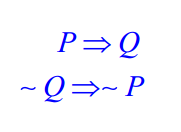
\includegraphics[scale=1]{logica.png}
\end{center}


\section{Condiciones suficientes: Las Condiciones de Cauchy-Riemann}

Ya se vio una condici\'on necesaria de diferenciabilidad, pero no suficiente. Completaremos este an\'alisis solicitando a la funci\'on que cumpla con un par de requisitos m\'as y con ello le daremos el alta. Les presentamos: \textbf{las Condiciones de Cauchy-Riemann}, que engloban las ecuaciones de Cauchy-Riemann.\\

\colorbox{green!40!white!80}{\parbox{\linewidth}{
\theoremstyle{theorem}
\begin{theorem} {Condiciones Suficientes}

Sea $f: S \subset \mathbb{C} \rightarrow \mathbb{C}$, con $f(z_0) = u(x_0, y_0) + i\cdot v(x_0, y_0)$ en donde $z_0 = x_0+iy_0$.\\

Si se cumple que:
\begin{enumerate}
	\item Existen las derivadas parciales de primer orden de $u(x, y)$ y de $v(x, y)$ en el entorno $\eta ((x_0, y_0), \rho)$
	\item Las derivadas parciales de primer orden de $u(x, y)$ y de $v(x, y)$ son continuas en $(x_0, y_0)$
	\item Dichas derivadas parciales cumplen con las Ecuaciones de Cauchy-Riemann $$u_x = v_y$$ $$u_y = -v_x$$
\end{enumerate}

entonces $f(z)$ es diferenciable en $(x_0, y_0)$

\end{theorem}}}
\linebreak

Demostrar\\

En s\'intesis, le sumamos a las ecuaciones de Cauchy-Riemann la \textbf{existencia} y \textbf{continuidad} de las derivadas parciales de $u$ y de $v$ y con ello tenemos condiciones suficientes de diferenciabilidad.\\


	\subsection{La versi\'on Polar}
	Hay circunstancias en las que una funci\'on $f(z)$ determinada es m\'as f\'acil expresarla como $f(z)=u(r, \theta) + i\ v(r, \theta)$, es decir, con funciones componentes que dependan de su m\'odulo y argumento, en vez de la parte real e imaginaria de $z$. Esto suceder\'a cuando la descomposici\'on de la funci\'on sea m\'as sencilla al representar a $z$ en su forma polar $z= r\ e^{i\theta}$.
	
	En caso de que tengamos una funci\'on expresada como $f(z)=u(r, \theta) + i\ v(r, \theta)$, no debemos entrar en p\'anico a la hora de tener que aplicar las ecuaciones de Cauchy-Riemann, ya que las mismas presentan un equivalente para la coordenadas polares.
	
	$$u_r = \frac{1}{r}v_{\theta}$$
	$$\frac{1}{r}u_{\theta} = -v_r$$
	
Bas\'andonos en la validez de la \textbf{forma polar de las ecuaciones de Cauchy-Riemann}, tenemos el siguiente teorema:\\

\colorbox{green!40!white!80}{\parbox{\linewidth}{
\theoremstyle{theorem}
\begin{theorem} {Condiciones de Cauchy-Riemann para coordenadas polares}

Sea $f(z) = u(r, \theta) + i\  v(r, \theta)$ una funci\'on definida en todos los puntos de un $\varepsilon$ entorno alrededro de un punto $z_0 = r_0\ e^{i\theta_0}$\\

Si se da que:
\begin{enumerate}
	\item las derivadas parciales de primer orden de $u(r, \theta)$ y $v(r, \theta)$ existen en todos los puntos del entorno
	\item tales derivadas son continuas en $(r_0, \theta_0)$
	\item tales derivadas cumplen con la forma polar de las ecuaciones de Cauchy-Riemann
	 $$u_r = \frac{1}{r}v_{\theta}$$ $$\frac{1}{r}u_{\theta} = -v_r$$
\end{enumerate}
...entonces la derivada $f'(z_0)$ existe.
\end{theorem}}}
\linebreak

Demostrar\\


En el caso del teorema anterior, la derivada de una funci\'on expresada de la forma $f(z) = u(r, \theta) + i\  v(r, \theta)$, viene dada por: $$f'(z) = e^{-i\theta}(u_r + i\ v_r)$$


\section{Analiticidad, aumentamos la exigencia}
Pareciese por capricho, pero llegados a esta altura, para seguir trabajando con c\'alculo complejo, no nos es suficiente que la funci\'on sea diferenciable en un punto. De ahora en adelante, nos vamos a sentir lo suficientemente c\'omodos para trabajar con funciones si \'estas son diferenciables no solamente en un punto $z_0$, sino que tambi\'en en sus alrededores, es decir, que lo sea tambi\'en en todo punto de alg\'un entorno $\eta$ centrado en $z_0$. Formalmente hablando... vamos a solicitar que $f(z)$ sea \textbf{anal\'itica} en $z_0$\\

\colorbox{blue!40!white!80}{\parbox{\linewidth}{
 \theoremstyle{definition}
 \begin{definition}{Analiticidad}

  	Sea $f: S \subset \mathbb{C} \rightarrow \mathbb{C}$. Diremos que $f$ es \textbf{anal\'itica} u \textbf{holomorfa} en $z_0 \in \mathbb{C}$ si existe la derivada de $f$ en $z_0$ y en alg\'un entorno centrado en $z_0$.
 \end{definition}}}
 \linebreak
 \linebreak

En base a la definici\'on anterior, diremos que $f(z)$ es \textbf{anal\'itica en un dominio} $\mathcal{S} \subset \mathbb{C}$ si es anal\'itica en todo punto de $\mathcal{S}$.

Tenemos entonces que la analiticidad es una condici\'on que no es \textit{puntual}, sino que es \textit{global}. Si una funci\'on $f(z)$ es anal\'itica en un punto $z_0$, entonces tambi\'en lo es en sus alrededores, pues que sea anal\'itica implica que sea derivable en un entorno $\eta$ centrado en $z_0$. Si es derivable en un entorno tal, todo punto en ese entorno estar\'a tambi\'en rodeado por puntos que sean derivables, siendo todos ellos puntos donde la funci\'on es anal\'itica.

Razonando de igual manera, tenemos que una funci\'on no puede ser anal\'itica en un punto $z_0$ aislado. En otras palabras, no puede ser anal\'itica en $z_0$ si no lo es en ning\'un otro punto de su cercan\'ia, o concretamente, en todo punto de alg\'un entorno de $z_0$.\\

\colorbox{blue!40!white!80}{\parbox{\linewidth}{
 \theoremstyle{definition}
 \begin{definition}{Funci\'on entera}

  	Si $f(z)$ es anal\'itica en todo $z \in \mathbb{C}$, entonces $f(z)$ se denomina una \textbf{funci\'on entera}.
 \end{definition}}}
\linebreak
\linebreak

Habiendo definido lo que es una funci\'on entera, cabe acotar que una funci\'on entera ser\'a para nosotros equivalente a lo que las funciones diferenciables en todo $\mathbb{R}^2$ son para el c\'alculo de varias variables. Ahora algunos teoremas.\\

\colorbox{blue!40!white!80}{\parbox{\linewidth}{
\theoremstyle{theorem}
\begin{theorem} {Analiticidad implica continuidad}

Sea $\mathcal{D}\subset \mathbb{C}$ un dominio complejo.

Si $f(z)$ es anal\'itica en $\mathcal{D}$, entonces $f(z)$ es continua en $\mathcal{D}$.

\end{theorem}}}
\linebreak
\linebreak

Algo interesante de la analiticidad es que, si una funci\'on es anal\'itica, lo ser\'a por siempre... o sea, no importa cu\'antas veces lo derives, su $n$-\'esima derivada ser\'a tambi\'en anal\'itica.\\

\colorbox{blue!40!white!80}{\parbox{\linewidth}{
\theoremstyle{theorem}
\begin{theorem} {Analiticidad de las derivadas}

Si una funci\'on $f(z)$ es anal\'itica en $z_0 \in \mathbb{C}$, sus derivadas de todos los \'ordenes son tambi\'en funciones anal\'iticas en $z_0$.

\end{theorem}}}
\linebreak
\linebreak

A continuaci\'on enunciamos algunas propiedades b\'asicas de la analiticidad. Sean $f, g$ dos funciones complejas de variable compleja, ambas anal\'iticas en el dominio complejo $\mathcal{D}$. Entonces: 
\begin{enumerate}
	\item $f + g$ es anal\'itica en $\mathcal{D}$
	\item $f \cdot g$ es anal\'itica en $\mathcal{D}$
	\item \mbox{\Large$\frac{f}{g}$} es anal\'itica en $\mathcal{D} - \{ z\: / \: g(z)=0\}$
	\item $f \circ g$ es anal\'itica en $\mathcal{D}$
\end{enumerate}

\section{Puntos Singulares}
Como anhelamos la analiticidad, y la analiticidad es una propiedad global, nos ser\'a de particular inter\'es discriminar aquellos puntos $z_0$ para los cuales, en medio de tanta analiticidad, la funci\'on \textit{no es anal\'itica}. Dichos puntos los conoceremos como \textbf{puntos singulares} o simplemente \textbf{singularidades}.\\

\colorbox{blue!40!white!80}{\parbox{\linewidth}{
 \theoremstyle{definition}
 \begin{definition}{Puntos singulares}

  	$z_0$ es un \textbf{punto singular} o una \textbf{singularidad} de $f(z)$ si $f$ no es anal\'itica en $z_0$ pero s\'i en alg\'un punto de todo entorno de $z_0$.
 \end{definition}}}
\linebreak
\linebreak

\colorbox{blue!40!white!80}{\parbox{\linewidth}{
 \theoremstyle{definition}
 \begin{definition}{Punto singular aislado}

  	$z_0$ es un \textbf{punto singular aislado} o una \textbf{singularidad aislada} de $f(z)$ si $f$ no es anal\'itica en $z_0$ pero s\'i en todo punto de alg\'un entorno reducido de $z_0$.
 \end{definition}}}
\linebreak

\begin{center}
	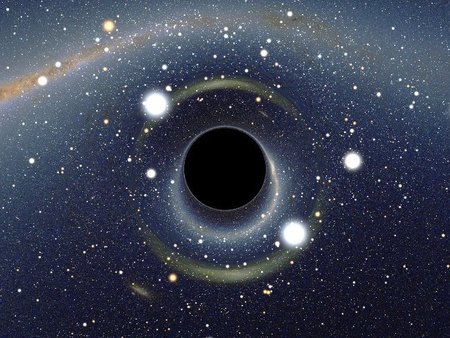
\includegraphics[scale=0.5]{singularidad.jpg}
\end{center}

\section{Funciones Arm\'onicas de $\mathbb{R}^2$}
Ahora frenamos un poquito y miramos para atr\'as... con atr\'as me refiero a las ya conocidas y visitadas funciones de varias variables reales. Existe cierta clase de funciones, real de dos variables reales, que se caracterizan simplemente por cumplir con la siguiente ecuaci\'on: $$\nabla^2f=0$$ Por ser as\'i de simple el requisito que se les solicita, las llamaremos \textbf{Funciones Arm\'onicas}.\\

\colorbox{yellow!40!white!80}{\parbox{\linewidth}{
 \theoremstyle{definition}
 \begin{definition}{Funciones Arm\'onicas}\\

  	Sea $\phi: \mathcal{D} \subset \mathbb{R}^2 \rightarrow \mathbb{R}$. Diremos que $\phi(x, y)$ es una \textbf{funci\'on arm\'onica} en $\mathcal{D}$ si:
  	\begin{itemize}
  		\item Las derivadas parciales primeras y segundas de $\phi$ \textbf{existen} y son \textbf{continuas} en $\mathcal{D}$.
  		\item La funci\'on $\phi(x, y)$ satisface la \textbf{Ecuaci\'on de Laplace:} $$\nabla^2 \phi = 0$$ $$\phi_{xx}(x, y) + \phi_{yy}(x, y) = 0$$
  	\end{itemize}
 \end{definition}}}
 \linebreak
 \linebreak

%\begin{multicols}{2}

\texttt{ATENCI\'ON}:

A no confundirse, que la catalogaci\'on de funci\'on arm\'onica se define para \textit{funciones de variable real}, concretamente para funciones que mapean valores de $\mathbb{R}^2$ a $\mathbb{R}$. NO para funciones de variable compleja. Este concepto nos sirve, sin embargo, para catalogar a las funciones componentes de una funci\'on compleja, que son en s\'i mismas funciones reales de dos variables reales.

\begin{center}
	
\includegraphics[scale=0.3]{armonia_musical.jpg}
\end{center}

%\end{multicols}

\colorbox{yellow!40!white!80}{\parbox{\linewidth}{
\theoremstyle{theorem}
\begin{theorem} {Analiticidad y armonicidad}
\\ \\
Sea $f : \mathcal{D}\subset \mathbb{C} \rightarrow \mathbb{C}$.

Si $f(z)=u(x, y) + i\ v(x, y)$ es anal\'itica en $\mathcal{D}$, entonces sus funciones componentes $u(x, y)$ y $v(x, y)$ son arm\'onicas en $\tilde{\mathcal{D}}\subset \mathbb{R}^2$

\end{theorem}}}
\linebreak
\linebreak

Dado el caso previo para la funci\'on $f(z)=u(x, y) + i\ v(x, y)$, se dice que la funci\'on $v(x, y)$ es \textbf{arm\'onica conjugada} de $u(x,y)$. De esta definici\'on, y del teorema anterior, encontramos !`oh sorpresa! que el que $v$ sea arm\'onica conjugada de $u$ es criterio suficiente para que la funci\'on $f(z)$ sea anal\'itica... wow, lo que es el poder de la armonicidad.\\

\colorbox{yellow!40!white!80}{\parbox{\linewidth}{
\theoremstyle{theorem}
\begin{theorem} {\ }
\\ \\
Sea $f : \mathcal{D}\subset \mathbb{C} \rightarrow \mathbb{C}$.

La funci\'on $f(z)=u(x, y) + i\ v(x, y)$ es anal\'itica en un dominio $\mathcal{D}$, si y s\'olo si $v(x, y)$ es arm\'onica conjugada de $u(x, y)$.

\end{theorem}}}
\linebreak
\linebreak











\end{document}